%% This is an example first chapter.  You should put chapter/appendix that you
%% write into a separate file, and add a line \include{yourfilename} to
%% main.tex, where `yourfilename.tex' is the name of the chapter/appendix file.
%% You can process specific files by typing their names in at the 
%% \files=
%% prompt when you run the file main.tex through LaTeX.
\chapter{Background and Related Work}
\section{Computer Musical Terminology}

\subsection{OMR}
OMR, or Optical Music Recognition, is method of recognizing the characters on scanned sheet music or printed scores and interpreting them into a digital form. 

\subsection{MIDI}
MIDI is the protocol with which electronic instruments and computers can communicate with each other. Many people associate MIDI with an idea of low-quality computer music, but it  just an instruction-like protocol, not actually a audio recording. At the basic level, MIDI messages encode notes with note-on, note-off times, and a number that corresponds to its frequency. A piece of music can be encoded in MIDI as a sequence of notes. On the other hand, MIDI files contain sequences of MIDI protocol events time-stamped for playback in a certain order.

\section{Non-musical Work in Sequence Alignment}
It is far easier to understand sequence alignment in a non-musical context (here the context is plain string alignment), understand the rules and assumptions made in the non-musical context, generalize them, and then recreate music-specific rules and assumptions. 

Readers familiar with the canonical representation of the string alignment problem as a dynamic programming matrix can skip this section. 

\subsection{An Overview of Sequence Alignment}
Sequence alignment in bioinformatics is an application of well-studied problem. In this field, researchers want to identify similar regions of DNA, RNA, or protein sequences to study functional, structural, or evolutionary relationships between the two sequences.

\begin{figure}[!ht]

\centering
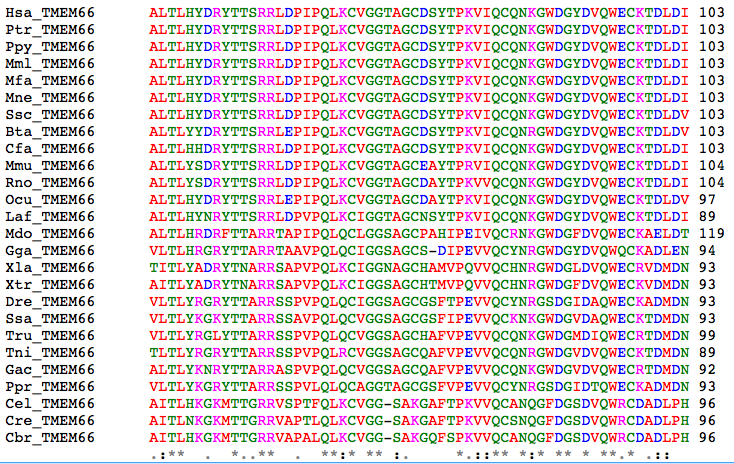
\includegraphics[scale=.5]{proteinalign}
\caption{An example of protein alignment \cite{proteins}}
\end{figure}

There are various computational algorithms that can be used to solve sequence alignment including slower but more accurate dynamic programming algorithms and faster but less accurate probabilistic or heuristic-based algorithms. In my work, it makes more sense to use the slower but more accurate methods, as our datasets are not so large and small mistakes that might be permissible to overlook in larger data could be much more egregious in smaller contexts.

The specific algorithm I chose to implement for solving the musical sequence alignment problem is a version of the Needleman-Wunsch dynamic programming algorithm for global sequence alignment. \footnote{This algorithm has a history of multiple invention. Needleman-Wunsch was first published in the context of protein alignment in bioinformatics. People with a more theoretical computer science bent might know the same algorithm by a different name, Wagner-Fisher.} 

At a high level, the Needleman-Wunsch algorithm and its family of dynamic programming sequence alignment algorithms calculate the edit distance between two sequences by producing a least-cost alignment of the sequences. An alignment is an assignment of pairwise characters and edit operations. Overall cost of an alignment (i.e. its \textbf{edit distance}) is determined by summing the individual costs of insertion, deletion, substitution, or no-change operations between pairwise characters in order to morph one sequence into the other. 

The next sections discuss coming up with edit distance calculations and then the method that Needleman-Wunsch uses to find the best alignment. 

\subsubsection{Edit Distance}

The term edit distance is a way of quantifying how dissimilar two sequences are to each other. If you think of sequences as being made up of characters, you can also think of one sequence transforming into the other through a series of insertion, deletion, substitution, and no-change operations, with each operation ''costing'' a certain amount. Edit distance is the smallest possible total cost associated with the transformation that is a series of operations that turns one sequence into another. As an example, consider the calculation of the edit distance between the two strings \textbf{MUSICAL} and \textbf{JUSTICE} that uses this series of operations for transforming \textbf{MUSICAL} into \textbf{JUSTICE}:

\begin{enumerate}
\item M $\rightarrow$  J (substitution)
\item $\epsilon \rightarrow$  T (insertion)
\item A $\rightarrow$  E (substitution)
\item L $\rightarrow  \epsilon$ (deletion)
\end{enumerate}


Note that implicitly I am excluding all the no-change operations that look like this:
\begin{enumerate}
\item U $\rightarrow$  U (no-change)
\end{enumerate}

\begin{table}[!h]
\centering
\begin{tabular}{ll}
\textbf{Operation} & \textbf{Cost} \\
Insertion          & 1             \\
Deletion           & 1             \\
Substitution       & 1             \\
No-change          & 0            
\end{tabular}
\caption{Naive Operation Cost Function Table}
\label{tab:naivetable}
\end{table}
	
This corresponds to an alignment that looks like figure \ref{best-alignment}. The green pair of characters indicate an insertion operation, red is deletion, and purple is substitution. These colors are also used in the visualization of OMR/MIDI stream alignment. 

\begin{figure}[!h]
\centering
\begin{tabular}{lcccccccccccc}
seq1 & {\color[HTML]{6200C9} \textbf{M}} & \textbf{U} & \textbf{S} & {\color[HTML]{009901} \textbf{\_}} & \textbf{I} & \textbf{C} & {\color[HTML]{6200C9} \textbf{A}} & {\color[HTML]{9A0000} \textbf{L}}  & \textbf{} & \textbf{} & \textbf{} &  \\
seq2 & {\color[HTML]{6200C9} \textbf{J}} & \textbf{U} & \textbf{S} & {\color[HTML]{009901} \textbf{T}}  & \textbf{I} & \textbf{C} & {\color[HTML]{6200C9} \textbf{E}} & {\color[HTML]{9A0000} \textbf{\_}} & \textbf{} & \textbf{} & \textbf{} & 
\end{tabular}
\caption{Alignment of MUSICAL and JUSTICE}
\label{best-alignment}
\end{figure}

The two strings have an edit distance of 4, because it requires four operations to completely morph one string into the other (discounting no-change operations).

However, one also might think that a substitution should ``cost'' more than either an insertion or deletion; after all, a substitution can be thought of as a consecutive insertion and deletion operation. 

A slightly different cost function that assigns more cost to substitution changes could look like table \ref{tab:naivetable2}. Using this cost function, the edit distance of changing \textbf{MUSICAL} into \textbf{JUSTICE} is 5.
\begin{table}[!h]
\centering
\begin{tabular}{ll}
\textbf{Operation} & \textbf{Cost} \\
Insertion          & 1             \\
Deletion           & 1             \\
Substitution       & 1.5             \\
No-change          & 0            
\end{tabular}
\caption{Operation Cost Table With Costlier Substitutions}
\label{tab:naivetable2}
\end{table}

But wait, should we certain subtypes of a single type of operation have differently weights? Consider if you were trying to run a spell checker (one application of string alignment and correction algorithms) on a word that wasn't recognized by the dictionary. In your particular spell check model, perhaps substitution of a vowel for a vowel isn't as costly as any other types of substitution. Let's say that substituting a vowel for a vowel should only have a cost of 1.2. Using this new cost function, the new edit distance is 4.7.
\begin{table}[!h]
\centering
\begin{tabular}{ll}
\textbf{Operation}             & \textbf{Cost} \\
Insertion                      & 1             \\
Deletion                       & 1             \\
Substitution - vowel for vowel & 1.2           \\
Substitution - all others      & 1.5           \\
No-change                      & 0                
\end{tabular}
\caption{Operation Cost Table With Different Substitution Costs}
\label{my-label3}
\end{table}

Considerations such as these go into the creation of a musical sequence aligner as well. 
\subsubsection{Alignment}

Recall that the edit distance between two sequences is defined as the least-cost alignment. Figure \ref{badalign} shows a valid alignment, but it is certainly not the least-cost alignment, and therefore does not correspond to the edit distance between between the two sequences, as it requires four substitutions, one insertion, and one deletion.

\begin{figure}[!h]
\centering
\begin{tabular}{lcccccccccccc}
seq1 & {\color[HTML]{009901} \textbf{\_}} & {\color[HTML]{6200C9} \textbf{M}} & {\color[HTML]{6200C9} \textbf{U}} & {\color[HTML]{6200C9} \textbf{S}} & \textbf{I} & \textbf{C} & {\color[HTML]{6200C9} \textbf{A}} & {\color[HTML]{9A0000} \textbf{L}}  & \textbf{} & \textbf{} & \textbf{} &  \\
seq2 & {\color[HTML]{009901} \textbf{J}}  & {\color[HTML]{6200C9} \textbf{U}} & {\color[HTML]{6200C9} \textbf{S}} & {\color[HTML]{6200C9} \textbf{T}} & \textbf{I} & \textbf{C} & {\color[HTML]{6200C9} \textbf{E}} & {\color[HTML]{9A0000} \textbf{\_}} & \textbf{} & \textbf{} & \textbf{} & 
\end{tabular}
\caption{A bad alignment of MUSICAL and JUSTICE}
\label{badalign}
\end{figure}

If there are two sequences, of length $n$ and $m$, then they have $\binom{n+m}{m}$ possible alignments. Put into context, consider two melodies of 10 notes each. Naively aligning just the note pitches, we have 184,765 different possible alignments! Clearly this isn't scalable, which is why we rely heavily on this piece of insight: A globally optimal alignment contains locally optimal alignments! This means that we can reuse the computations of subproblems to solve larger problems. What follows from this piece of insight is that for two strings split at $(i, j)$, the best alignment is:

\begin{center}
best alignment of \texttt{string1}$[:i]$ and \texttt{string2}$[:j]$ 
$+$ best alignment of \texttt{string1}$[i:]$ and \texttt{string2}$[j:]$
\end{center}

\begin{figure}[!h]`
\centering
\begin{tabular}{lccccccc}
   & {\color[HTML]{333333} \textbf{}} & \multicolumn{2}{c}{{\color[HTML]{333333} $i$}}          & {\color[HTML]{333333} \textbf{}} & {\color[HTML]{333333} \textbf{}} & {\color[HTML]{333333} \textbf{}} & {\color[HTML]{333333} \textbf{}} \\
   & {\color[HTML]{333333} \textbf{}} & \multicolumn{2}{c}{{\color[HTML]{333333} $\downarrow$}} & {\color[HTML]{333333} \textbf{}} & {\color[HTML]{333333} \textbf{}} & {\color[HTML]{333333} \textbf{}} & {\color[HTML]{333333} \textbf{}} \\
\texttt{seq1} & \textbf{M}                       & \textbf{U}                  & \textbf{S}                & \textbf{I}                       & \textbf{C}                       & \textbf{A}                       & \textbf{L}                       \\
\texttt{seq2} & \textbf{J}                       & \textbf{U}                  & \textbf{S}                & \textbf{T}                       & \textbf{I}                       & \textbf{C}                       & \textbf{E}                       \\
   &                                  &                             &                           &                                  & \multicolumn{2}{c}{$\uparrow$}                                      &                                  \\
   &                                  &                             &                           &                                  & \multicolumn{2}{c}{$j$}                                             &                                 
\end{tabular}
\caption{The alignment of MUSICAL split at \textit{i} and JUSTICE split at \textit{j}}
\label{indexed musical and justice}
\end{figure}

If we can keep track of all the possible alignment subproblems, we can recursively build an optimal solution using the answers from the subproblems. One way to represent this is with a scoring matrix indexed by $i$ and $j$. For the problem of aligning \textbf{MUSICAL} and \textbf{JUSTICE}, the setup would look something like the following.


\begin{figure}[!h]
\centering
\begin{tabular}{lllllllll}
                                & \multicolumn{1}{c}{\textbf{-}} & \textbf{J}            & \textbf{U}            & \textbf{S}            & \textbf{T}            & \textbf{I}            & \textbf{C}            & \textbf{E}            \\ \cline{2-9} 
\multicolumn{1}{c|}{\textbf{-}} & \multicolumn{1}{l|}{}          & \multicolumn{1}{l|}{} & \multicolumn{1}{l|}{} & \multicolumn{1}{l|}{} & \multicolumn{1}{l|}{} & \multicolumn{1}{l|}{} & \multicolumn{1}{l|}{} & \multicolumn{1}{l|}{} \\ \cline{2-9} 
\multicolumn{1}{l|}{\textbf{M}} & \multicolumn{1}{l|}{}          & \multicolumn{1}{l|}{} & \multicolumn{1}{l|}{} & \multicolumn{1}{l|}{} & \multicolumn{1}{l|}{} & \multicolumn{1}{l|}{} & \multicolumn{1}{l|}{} & \multicolumn{1}{l|}{} \\ \cline{2-9} 
\multicolumn{1}{l|}{\textbf{U}} & \multicolumn{1}{l|}{}          & \multicolumn{1}{l|}{} & \multicolumn{1}{l|}{} & \multicolumn{1}{l|}{} & \multicolumn{1}{l|}{} & \multicolumn{1}{l|}{} & \multicolumn{1}{l|}{} & \multicolumn{1}{l|}{} \\ \cline{2-9} 
\multicolumn{1}{l|}{\textbf{S}} & \multicolumn{1}{l|}{}          & \multicolumn{1}{l|}{} & \multicolumn{1}{l|}{} & \multicolumn{1}{l|}{} & \multicolumn{1}{l|}{} & \multicolumn{1}{l|}{} & \multicolumn{1}{l|}{} & \multicolumn{1}{l|}{} \\ \cline{2-9} 
\multicolumn{1}{l|}{\textbf{I}} & \multicolumn{1}{l|}{}          & \multicolumn{1}{l|}{} & \multicolumn{1}{l|}{} & \multicolumn{1}{l|}{} & \multicolumn{1}{l|}{} & \multicolumn{1}{l|}{} & \multicolumn{1}{l|}{} & \multicolumn{1}{l|}{} \\ \cline{2-9} 
\multicolumn{1}{l|}{\textbf{C}} & \multicolumn{1}{l|}{}          & \multicolumn{1}{l|}{} & \multicolumn{1}{l|}{} & \multicolumn{1}{l|}{} & \multicolumn{1}{l|}{} & \multicolumn{1}{l|}{} & \multicolumn{1}{l|}{} & \multicolumn{1}{l|}{} \\ \cline{2-9} 
\multicolumn{1}{l|}{\textbf{A}} & \multicolumn{1}{l|}{}          & \multicolumn{1}{l|}{} & \multicolumn{1}{l|}{} & \multicolumn{1}{l|}{} & \multicolumn{1}{l|}{} & \multicolumn{1}{l|}{} & \multicolumn{1}{l|}{} & \multicolumn{1}{l|}{} \\ \cline{2-9} 
\multicolumn{1}{l|}{\textbf{L}}   & \multicolumn{1}{l|}{}          & \multicolumn{1}{l|}{} & \multicolumn{1}{l|}{} & \multicolumn{1}{l|}{} & \multicolumn{1}{l|}{} & \multicolumn{1}{l|}{} & \multicolumn{1}{l|}{} & \multicolumn{1}{l|}{} \\ \cline{2-9} 
\end{tabular}
\caption{Initial distance matrix setup for aligning MUSICAL and JUSTICE}
\label{alignsetup}
\end{figure}

Recall that we have defined the problem in three different ways:
\begin{enumerate}
\item Aligning \textbf{MUSICAL} and \textbf{JUSTICE}
\item Finding the edit distance between \textbf{MUSICAL} and \textbf{JUSTICE}
\item Finding a series of operations that transforms \textbf{MUSICAL} into \textbf{JUSTICE}
\end{enumerate}

All of these problem definitions are (almost) one and the same. Calculating the edit distance will also provide a good alignment of the two words and a good alignment necessitates a series of character change operations. It is important to know that that (3) has an implicit directionality built into the problem statement. It won't always be the case that alignments and transformations are symmetric (i.e. cost the same and have the same series of operations), but having a simple cost operation functions, such as in tables 
\ref{tab:naivetable}
 and 
 \ref{tab:naivetable2} 
 will make such problems symmetric. 

In this particular sample problem, we will always be transforming one word, \textbf{MUSICAL} into another, \textbf{JUSTICE}. In the context of my thesis, we will always be transforming OMR sequences in MIDI sequences. 

After we've set up is the scoring matrix, we will populate it with initial values: 
\begin{enumerate}
\item 0 in $(0,0)$
\item $i-1 \cdot insertion cost$ for $i$ in $(i, 0)$ (this is the first column) 
\item $j-1 \cdot deletion cost$ for $j$ in $(0, j)$ (this is the first column) 
\end{enumerate}
In reading a scoring matrix setup like this, insertions are vertical movements, deletions are horizontal movements, and substitutions are diagonal. 
After we've set up the initial matrix, we can go through and fill in all of the remaining slots using this update rule:


\begin{equation*}
\begin{split}
\text{D[i][j]} = &  \text{min \{ }\\
& \text{D[i-1][j] + insCost (),} \\
& \text{D[i][j-1] + delCost,} \\
& \text{D[i-1][j-1] + subCost} \\
\text{\}}
\end{split}
\end{equation*}


\section{Turning Sequence Alignment into a Musical Problem}
Finding the edit distance of a musical sequence as opposed to a string of ASCII characters is a little trickier. First, there isn?t an intuitive ''space'' of music elements the way that there is a ''space'' of all characters. Second, even after identifying the musical elements, there isn?t an intuitive metric of distance between elements. For example, how would the distance between [Ab quarter note, 4th octave] and [Bb quarter note, 4th octave] compare with [Ab either note, 4th octave] and [Ab quarter note, 4th octave]? [pictures, maybe an even more ambiguous example]

Going back to [original model] and the questions we posed and answered for string alignment, 

\begin{itemize}
\item What sequences are and what makes them up: We can think of musical sequences as an ordering of notes, rests, and chords
\item The space that sequences occupy: This question can roughly be approximated as, what properties of notes, rests, chords do we care about? Some immediate answers are pitch, duration, rhythm.
\item Coming up with an appropriate metric for finding distance: In the previous section we had two different substitution functions. What kind of and how many ways do we want to calculate distance in musical elements?
\end {itemize}


\section{Related Work}
\subsection{Typke: Music Retrieval based on Melodic Similarity}
Another instance in which music is transformed and compressed into its most relevant features before comparison is in Typke's thesis on Music Retrieval based on Melodic Similarity \cite{typke}. Here, Typke proposes encoding music into what he calls a ``weighted point set" in a two-dimensional space of time and pitch before measuring any sort of melodic similarity between music. A note in a piece is represented as point set of pitch (in the Hewlett 40 system \cite{typke}) and an offset in quarter notes from the beginning of the piece.

\subsection{Church and Cuthbert: Rhythmic Comparison and Alignment}
Church and Cuthbert \cite{church} describe a system that hashes scores purely on rhythm and uses heuristics of rhythm in music (e.g. a repeated rhythm should be the same every time it is expected to repeat) to correct OMR scores. I believe that this model could be built upon with the hasher object in tandem with more heuristics pertaining to the qualities of music that I hash to further improve OMR accuracy.

\subsection{Viro: Peachnote, Musical Score Search and Analysis and IMSLP}
Peachnote \cite{peachnote} and IMSLP \cite{imslp} both are projects that contain large bodies of musical scores. Peachnote performs a search of a musical phrase and tends to introduce errors in chord progression searches that requires recognition of musical staves. IMSLP holds a large collection of musical scores. many of which are user contributed (i.e. not necessarily ground truth). Both of these bodies of work contain information about musical scores that my work can draw upon and use. 

\subsection{White: Statistical Properties of Music and MIDI}
White's dissertation \cite{white} describes properties of music that can be turned into heuristics for refining algorithmic analysis of music. Specifically, he builds upon Temperley's 1997 \cite{temperley} paper's details to harmonic analysis of MIDI and refers to other research that has been constructive towards Temperley's model. White does say that Temperley's algorithm fails when faced with ambiguity, such as in MIDI differentiating between enharmonic tones. The hope is that by combining the ambiguous parts of MIDI with the probabilistic and rigorous details of OMR scores, ambiguities in MIDI tonality can be resolved. In addition, White also cites a large repository of high quality MIDI files. 

\subsection{Rebelo et al: Optical Music Recognition - State-of-the-Art and Open Issues}
Rebelo et al's paper discusses the state of the art of OMR at each step of the OMR process and proposes future work in certain areas that would advance the current state of OMR. 
\cite{rebelo}

\subsection{OpenScore}
OpenScore is project